
Rossby-Wellen, auch planetare Wellen genannt, sind grossräumige
Wellenerscheinungen, die in erster Linie durch die Breitenabhängigkeit des
Coriolis-Parameters verursacht werden. Diese Breitenabhängigkeit wird durch den
sogenannten \emph{Beta-Term}
\begin{equation}
	\beta = \frac{\partial f}{\partial y}
	\label{rossby:eq:beta_term}
\end{equation}
beschrieben. Bewegt sich ein Luftpaket meridional, erfährt es eine Änderung seiner planetaren Vorticity \(f\). Unter der Erhaltung der potenziellen Vorticity erzwingt dies eine kompensierende Änderung der relativen Vorticity~\(\zeta\), was zu einer wellenförmigen Rückstellbewegung führt.
Diese Dynamik macht Rossby-Wellen zu einer direkten Konsequenz der Erhaltung der potenziellen Vorticity auf einer Kugel oder \(\beta\)-Ebene.

\subsubsection{Lineare Theorie barotroper Rossby-Wellen}

Abschnitt inspiriert von \cite{rossby:mueller2018}.

In Äquatornähe dominiert eine mittlere Ost–West-Strömung mit Geschwindigkeit
\(U\). Betrachten wir kleine Störungen \((u,v)\) dieser Strömung:
\begin{equation}
	u' = U + u, \quad v' = v, \quad \text{mit } |u|, |v| \ll U.
	\label{rossby:eq:perturbation}
\end{equation}
Für eine quellenfreie Strömung existiert eine Stromfunktion~$\psi$ (vgl.~Abschnitt~\ref{ueberschall:stroemungsgleichung}):
\begin{equation}
	u = -\frac{\partial \psi}{\partial y}, \quad v = \frac{\partial \psi}{\partial x}.
	\label{rossby:eq:stream_function}
\end{equation}
Die relative Vorticity ergibt sich zu
\begin{equation}
	\zeta = \frac{\partial v}{\partial x} - \frac{\partial u}{\partial y} = \Delta \psi,
	\label{rossby:eq:relative_vorticity}
\end{equation}
und die absolute Vorticity ist \(\zeta + f\) mit \(f = f(y)\). Unter der Annahme, dass die absolute Vorticity in der reibungsfreien Strömung erhalten bleibt,
\begin{equation}
	\frac{d}{dt} (\zeta + f) = 0,
	\label{rossby:eq:absolute_vorticity_conservation}
\end{equation}
und unter Verwendung der Näherungen
\begin{equation}
	u \ll U, \quad \frac{\partial \zeta}{\partial y} \ll \frac{\partial f}{\partial y} = \beta, \quad v = \frac{\partial \psi}{\partial x},
	\label{rossby:eq:linear_approximations}
\end{equation}
erhält man die linearisierte Vorticity-Gleichung
\begin{equation}
	\frac{\partial \zeta}{\partial t} + U \frac{\partial \zeta}{\partial x} + \beta \frac{\partial \psi}{\partial x} = 0.
	\label{rossby:eq:linear_vorticity_equation}
\end{equation}
Mit \(\zeta = \Delta \psi\) folgt
\begin{equation}
	\frac{\partial \Delta \psi}{\partial t} + U \frac{\partial \Delta \psi}{\partial x} + \beta \frac{\partial \psi}{\partial x} = 0.
	\label{rossby:eq:linear_vorticity_equation_psi}
\end{equation}

\subsubsection{Wellenlösung und Dispersionsrelation}

Wir setzen eine ebene Welle der Form
\begin{equation}
	\psi(x,y,t) = \cos(kx + ly - \omega t)
	\label{rossby:eq:wave_solution}
\end{equation}
ein und erhalten die Dispersionsrelation
\begin{equation}
	\omega = U k - \frac{\beta k}{k^2 + l^2}.
	\label{rossby:eq:dispersion_relation}
\end{equation}
Die Phasengeschwindigkeit lautet
\begin{equation}
	c = \frac{\omega}{k} = U - \frac{\beta}{k^2 + l^2}.
	\label{rossby:eq:phase_speed}
\end{equation}
Daraus folgt, dass sich Rossby-Wellen relativ zur mittleren Strömung stets nach Westen ausbreiten. In der Atmosphäre bedeutet dies: Selbst bei einer nach Osten gerichteten Grundströmung (z. B. im Jetstream) bewegt sich die Wellenform gegen die Strömung. Rossby-Wellen sind besonders stabil und können über viele Tage bestehen, wodurch sie grossräumig die Lage von Hoch- und Tiefdrucksystemen und die Pfade von Wetterfronten beeinflussen.

\subsection{Rossby-Wellen und Wetterextreme}



\begin{figure}
	\centering
	\renewcommand{\arraystretch}{0.5}
	\begin{tabular}{ccc}
		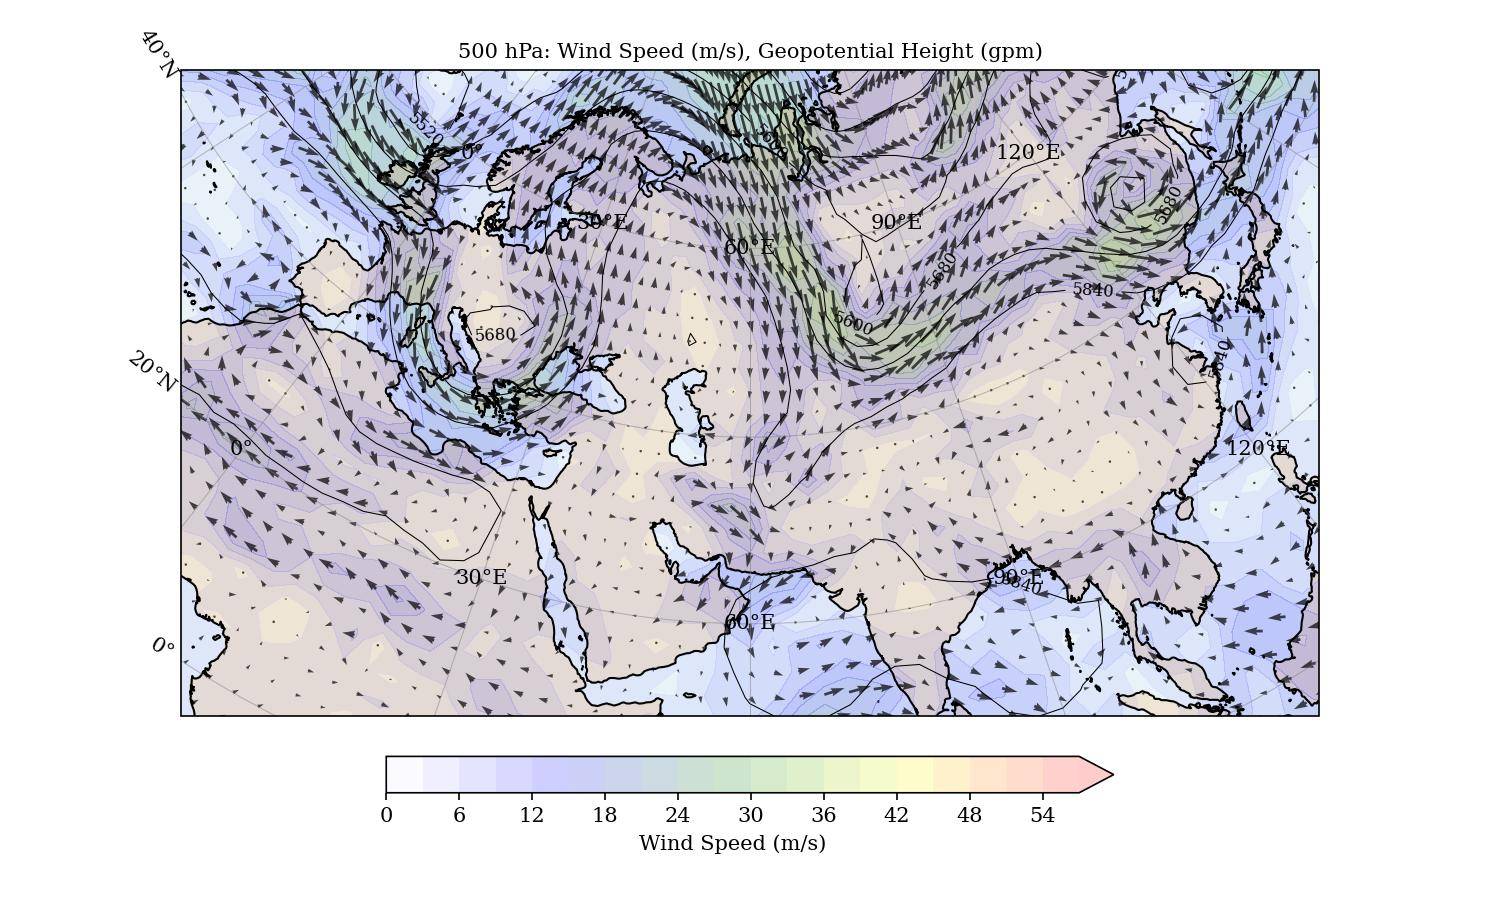
\includegraphics[width=0.32\textwidth, trim=3cm 3cm 3cm 1.1cm, clip]{papers/rossby/images/data_2010_7_27_12_00_500.jpg} &
		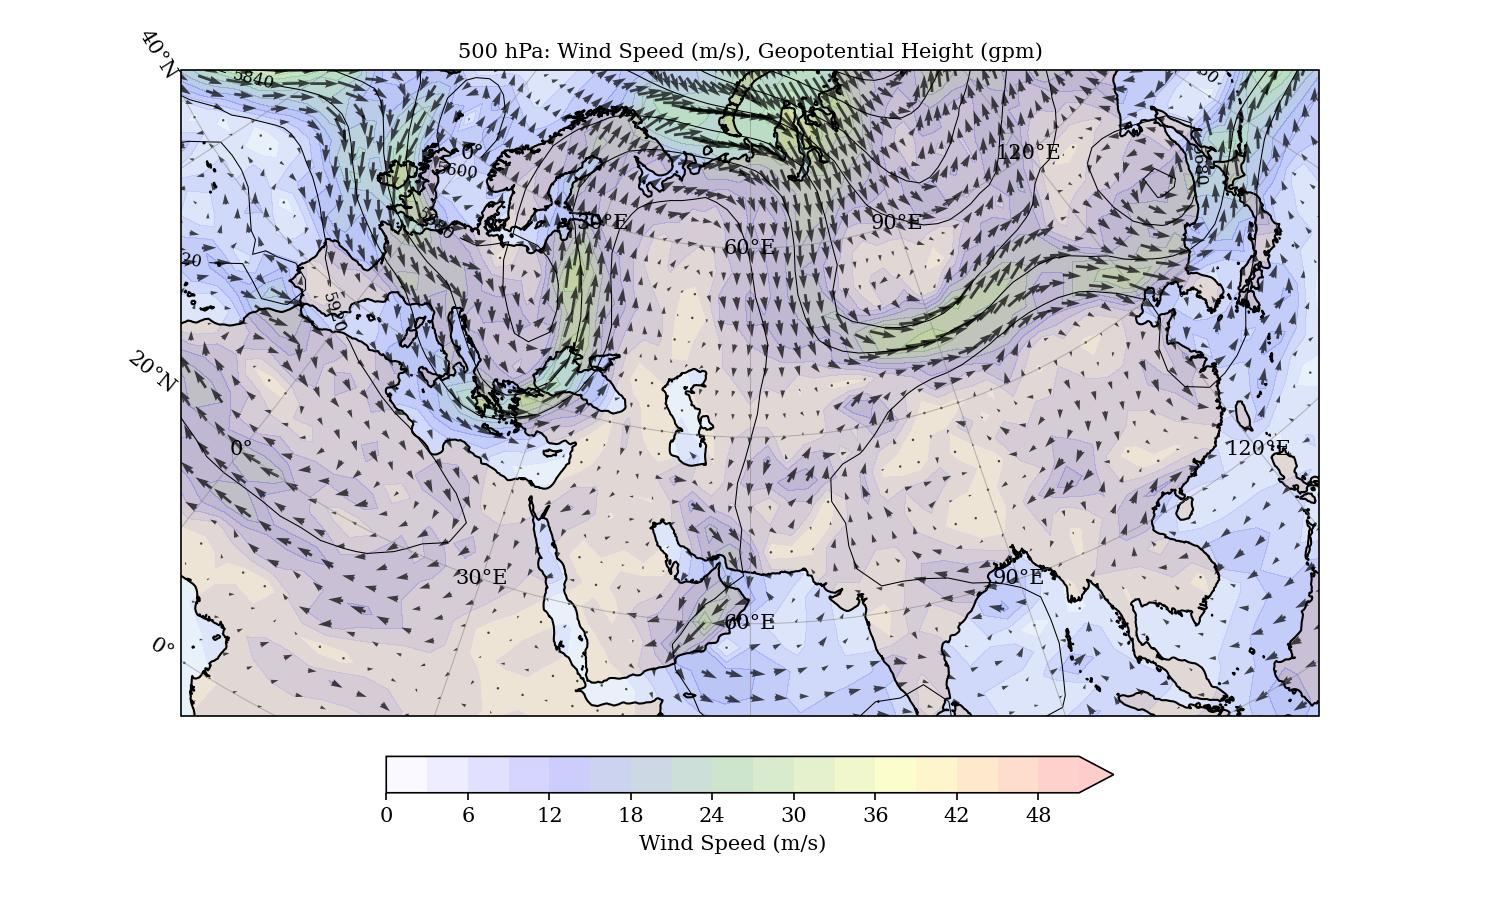
\includegraphics[width=0.32\textwidth, trim=3cm 3cm 3cm 1.1cm, clip]{papers/rossby/images/data_2010_7_28_12_00_500.jpg} &
		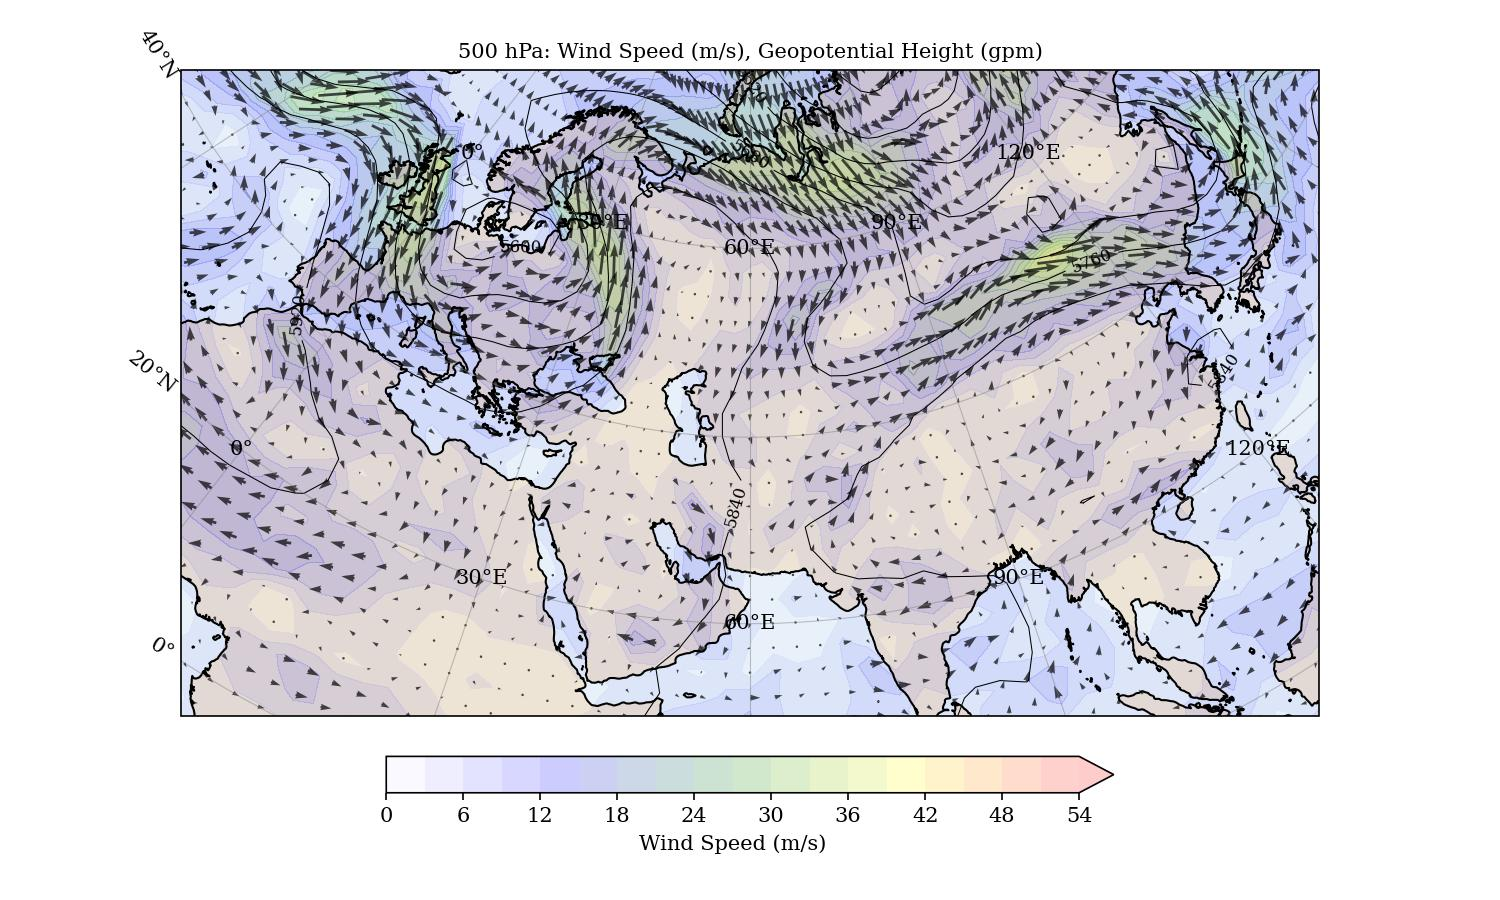
\includegraphics[width=0.32\textwidth, trim=3cm 3cm 3cm 1.1cm, clip]{papers/rossby/images/data_2010_7_29_12_00_500.jpg}   \\
		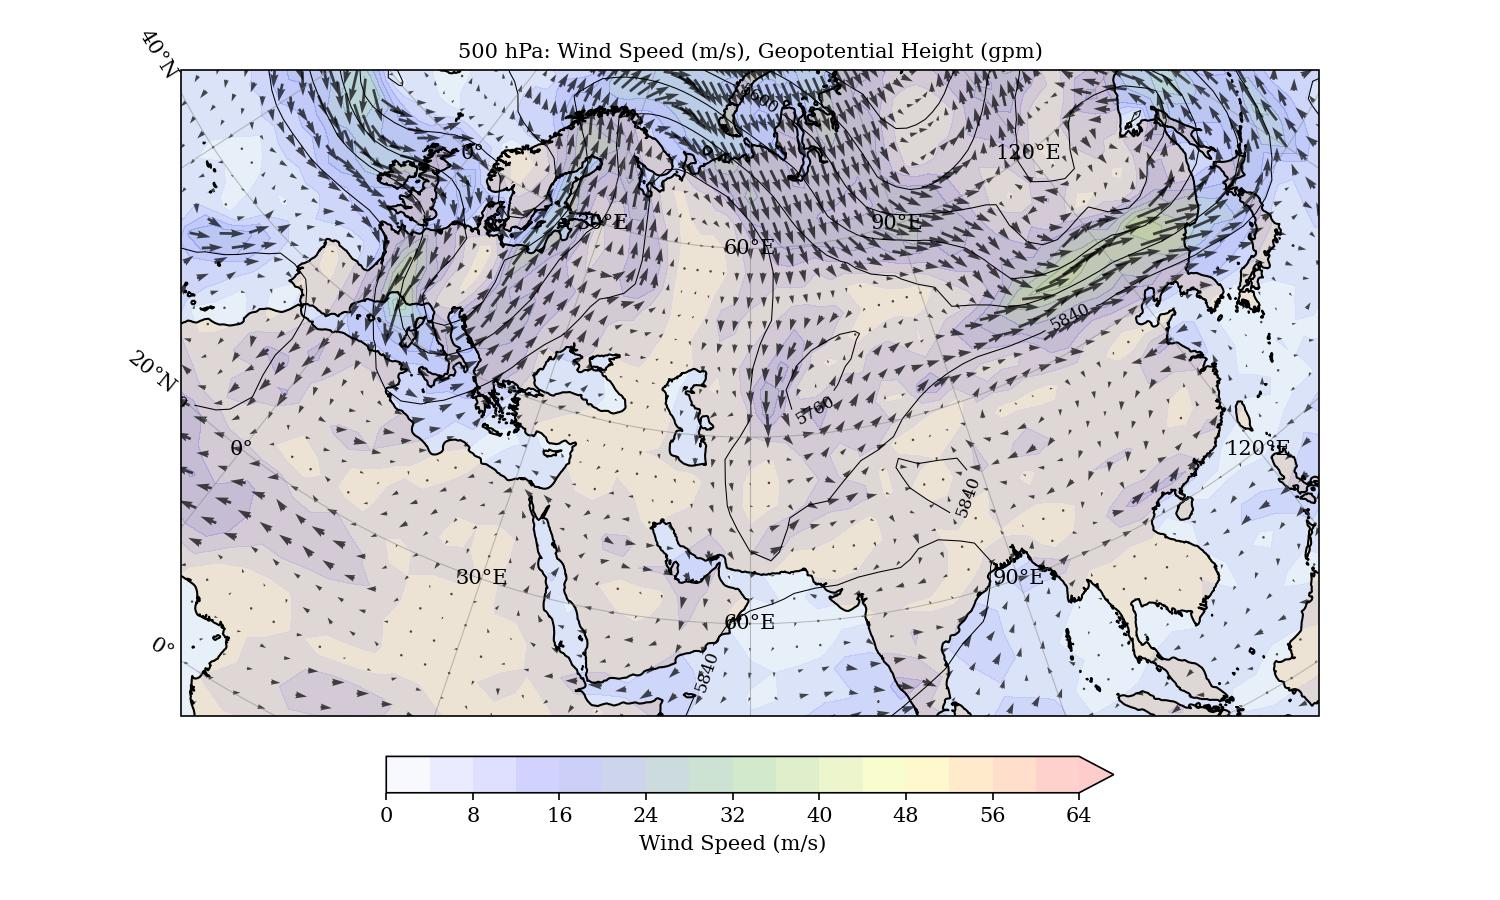
\includegraphics[width=0.32\textwidth, trim=3cm 3cm 3cm 1.1cm, clip]{papers/rossby/images/data_2010_7_30_12_00_500.jpg} &
		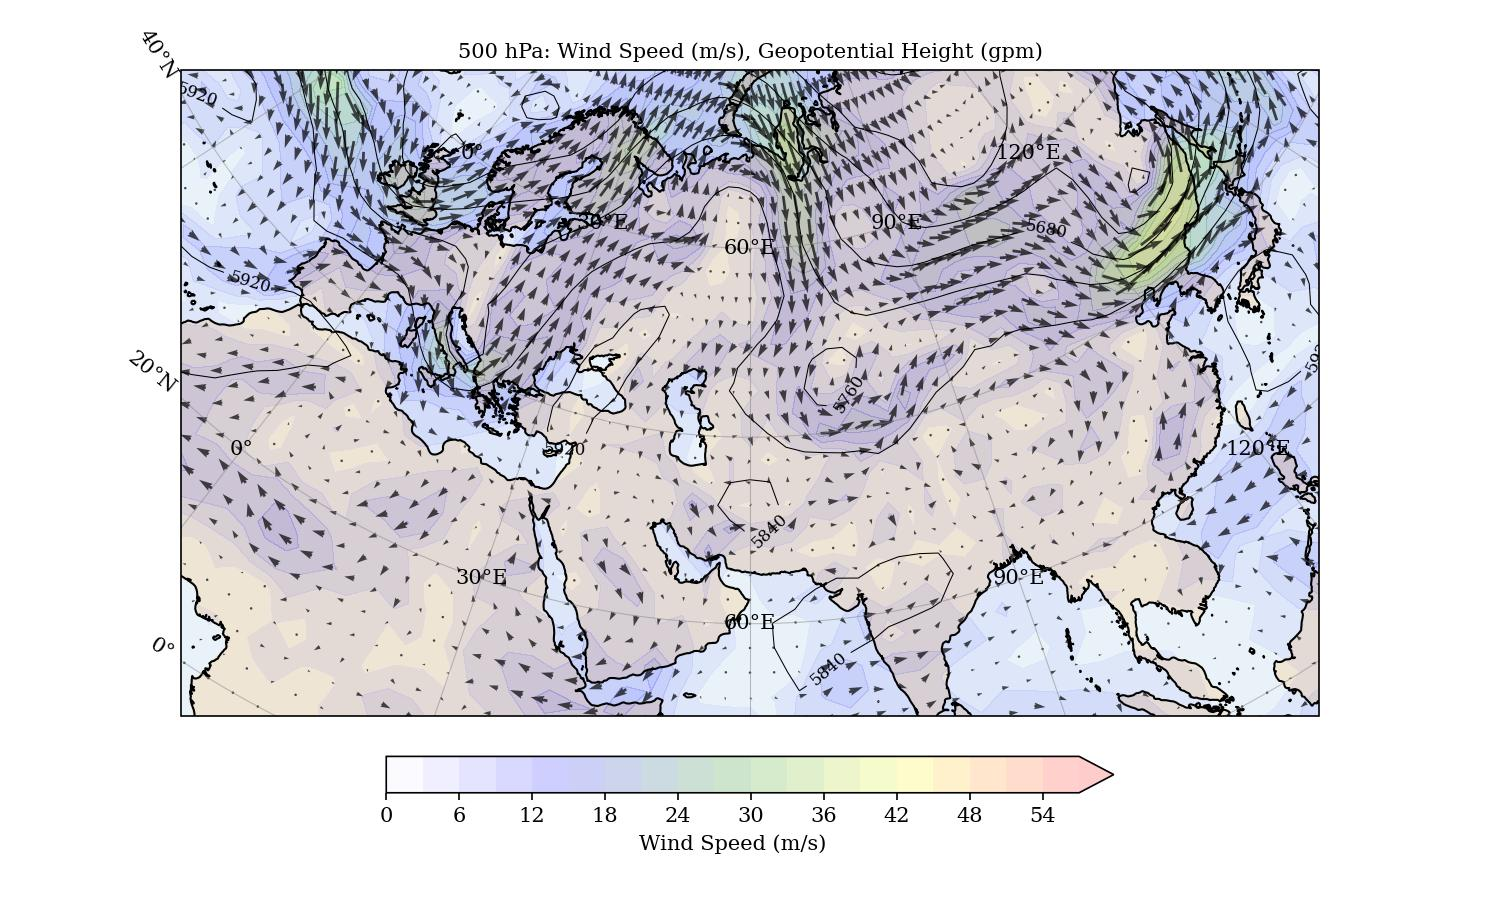
\includegraphics[width=0.32\textwidth, trim=3cm 3cm 3cm 1.1cm, clip]{papers/rossby/images/data_2010_7_31_12_00_500.jpg} &
		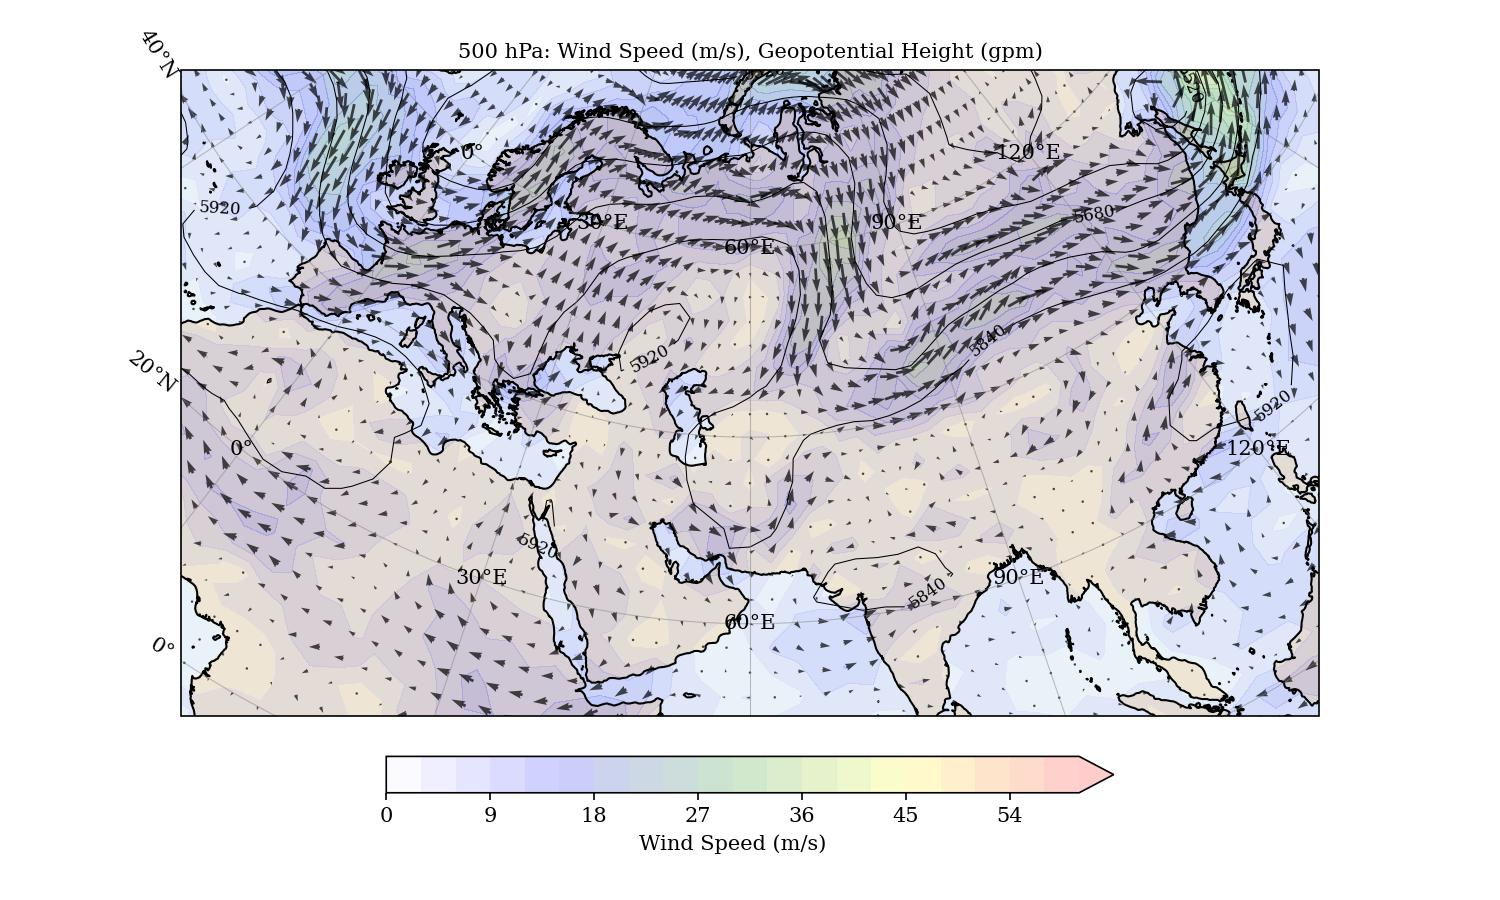
\includegraphics[width=0.32\textwidth, trim=3cm 3cm 3cm 1.1cm, clip]{papers/rossby/images/data_2010_8_1_12_00_500.jpg}   \\
		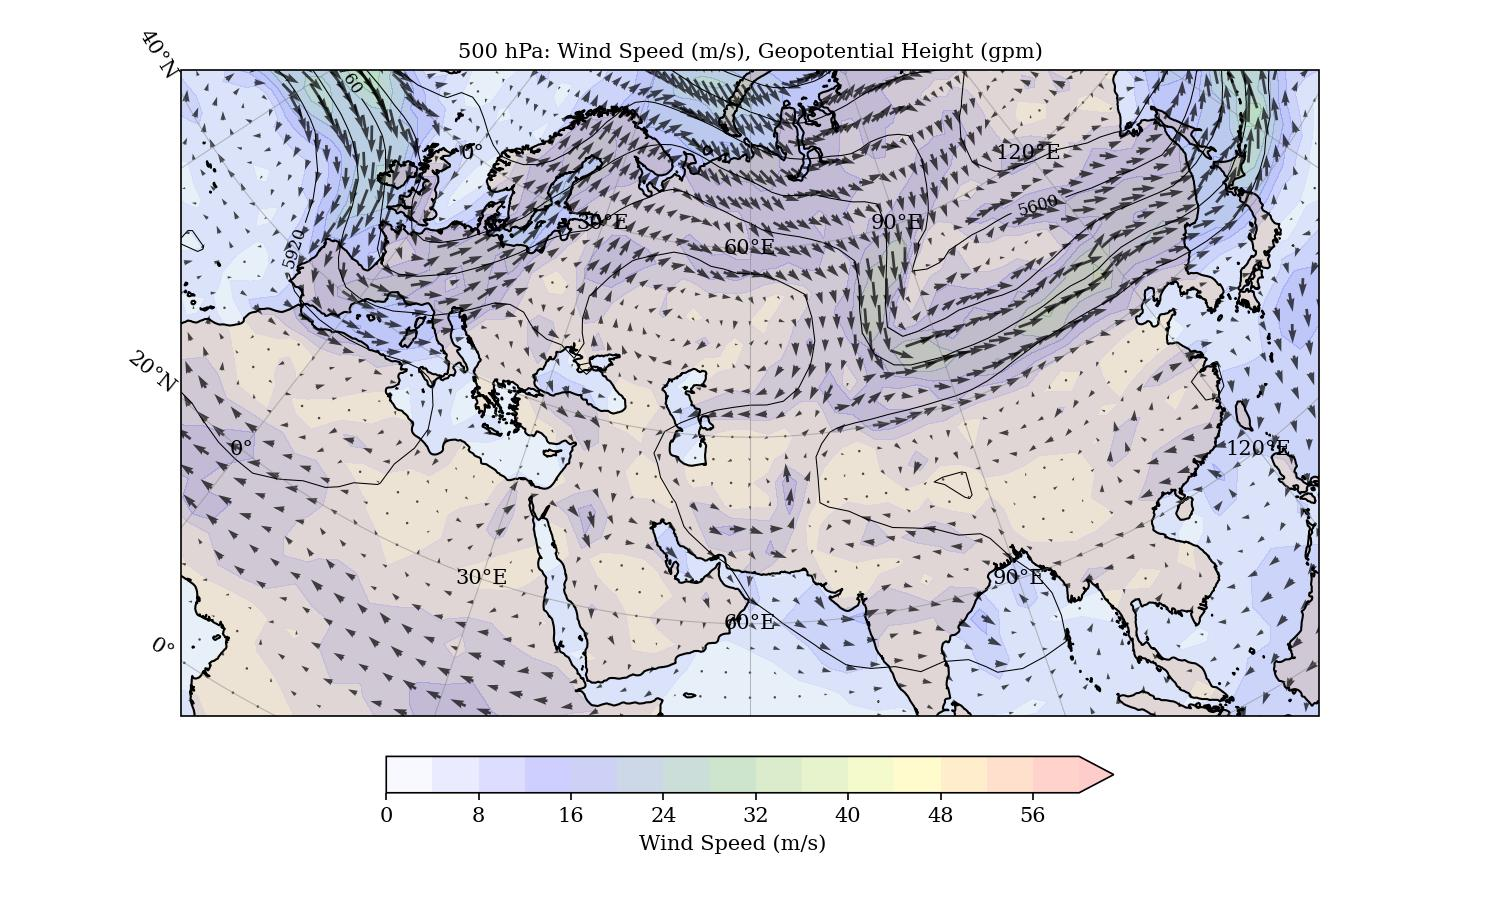
\includegraphics[width=0.32\textwidth, trim=3cm 3cm 3cm 1.1cm, clip]{papers/rossby/images/data_2010_8_2_12_00_500.jpg} &
		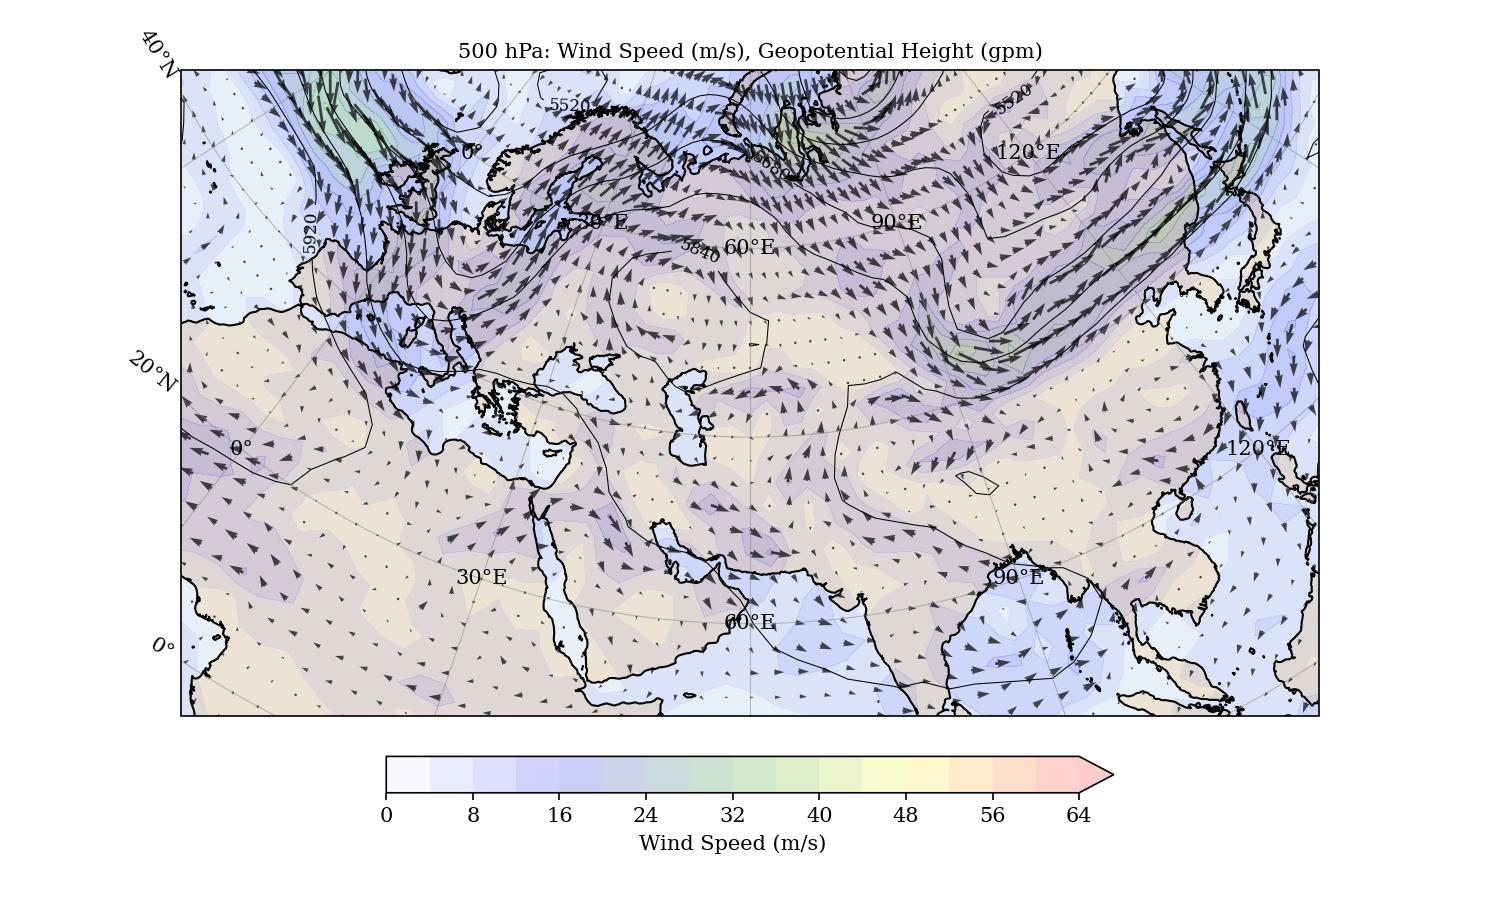
\includegraphics[width=0.32\textwidth, trim=3cm 3cm 3cm 1.1cm, clip]{papers/rossby/images/data_2010_8_3_12_00_500.jpg} &
		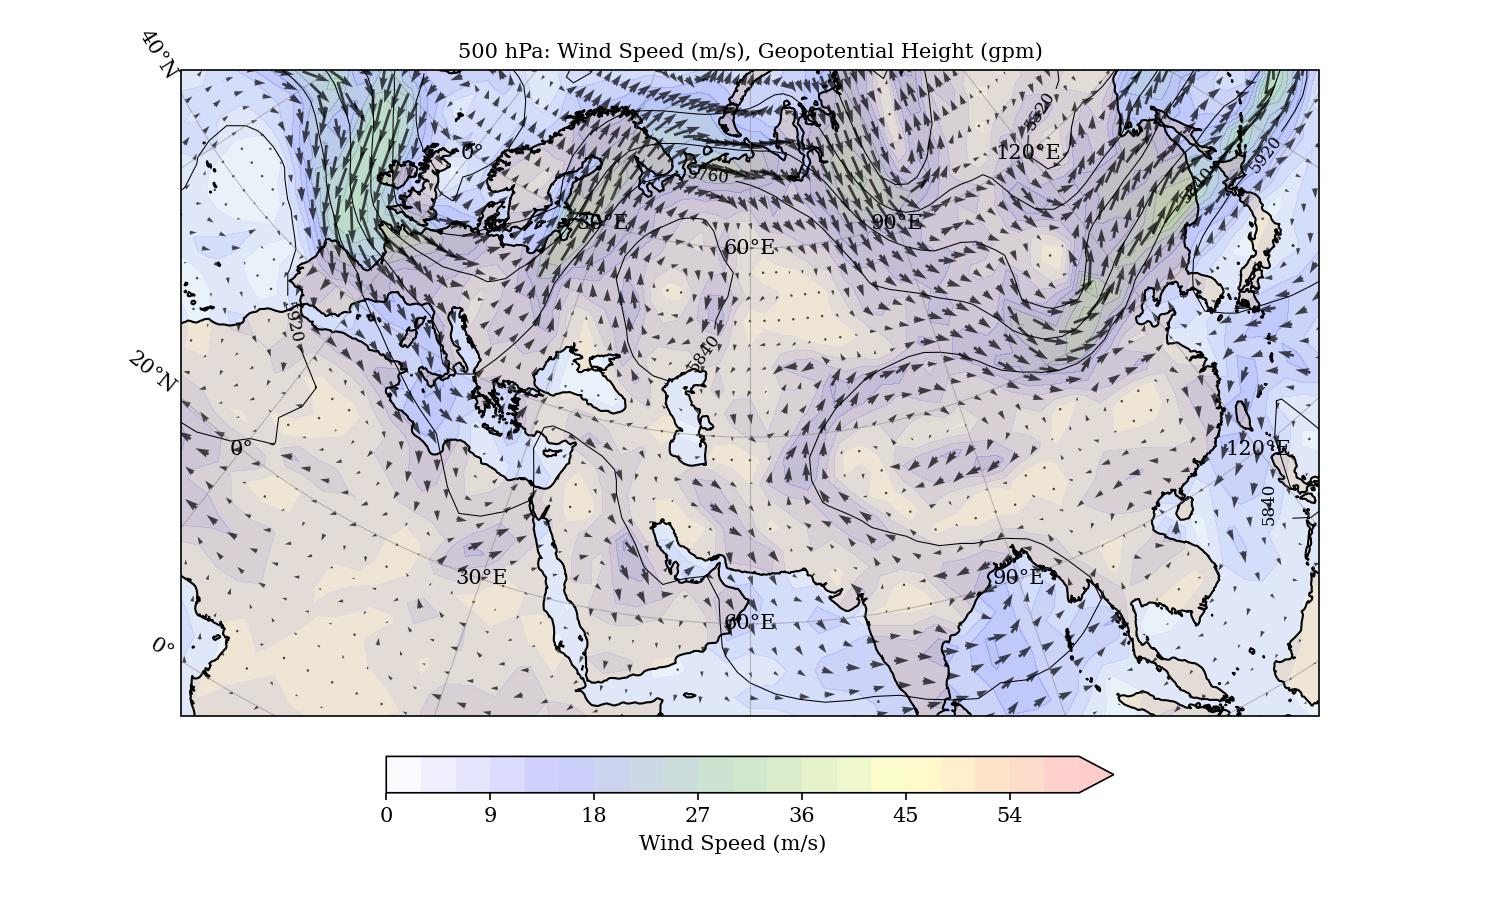
\includegraphics[width=0.32\textwidth, trim=3cm 3cm 3cm 1.1cm, clip]{papers/rossby/images/data_2010_8_4_12_00_500.jpg}   \\
	\end{tabular}
	\caption{Abfolge der Rossby-Wellenstruktur in 500\,hPa Höhe vom 27. Juli bis 4.\ August 2010 in 24-Stunden-Schritten.
	Die Ansicht zeigt den Kontinet Aisen, die We
		Die Teilabbildungen sind zeilenweise von links nach rechts zu lesen, beginnend mit dem 27.\ Juli 12:00~UTC (oben links)
		bis zum 4.\ August 12:00~UTC (unten rechts).}
	\label{fig:rossby_grid_2010}
\end{figure}


Ein eindrucksvolles Beispiel für den Einfluss quasi-stationärer Rossby-Wellen
auf Extremwetterereignisse ist der Sommer 2010. In dieser Periode dominierten
atmosphärische Zirkulationsmuster mit einer Wellenzahl \(k \approx 6 - 8\), die zu
gleichzeitigen, aber geographisch weit entfernten Extremen führten, siehe auch Abbildung \ref{fig:rossby_2010}.


\begin{figure}
	\centering
	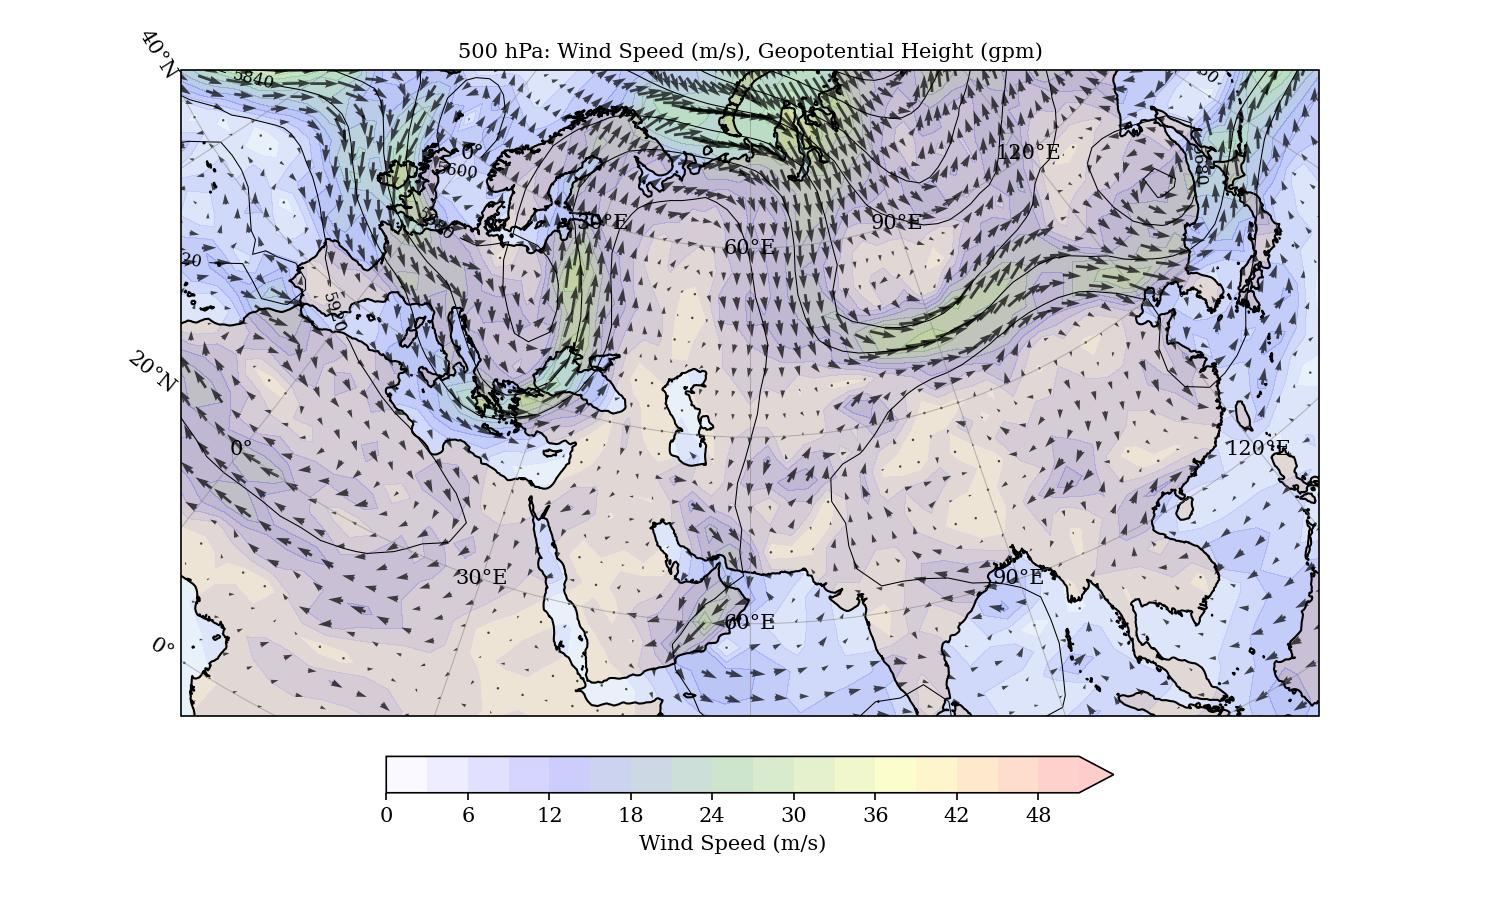
\includegraphics[width=\textwidth, trim=2cm 0cm 3cm 0cm, clip]{papers/rossby/images/data_2010_7_28_12_00_500.jpg}
	\caption{500\,hPa Windfeld am
		28.\ Juli 2010, 12:00~UTC, während der gleichzeitigen Flutereignisse in Pakistan und
		der Hitzewelle in Russland. Die Abbildung zeigt eine charakteristische Rossby-Wellenstruktur,
		die über einen längeren Zeitraum stabil blieb.}
	\label{fig:rossby_2010}
\end{figure}


Über Westrussland etablierte sich ein blockierendes Hochdruckgebiet, das über Wochen bestehen blieb und eine extreme Hitzewelle mit Temperaturen über 40\,$^\circ$C auslöste.
Die anhaltende Trockenheit begünstigte grossflächige Waldbrände und dichten Smog, besonders im Raum Moskau, mit tausenden Todesopfern.

Zur gleichen Zeit erlebte Pakistan ungewöhnlich starken Monsunregen. Ein
persistentes Tiefdruckgebiet führte zu einer Jahrhundertflut, von der über 20
Millionen Menschen betroffen waren.

Beide Ereignisse lassen sich durch dasselbe planetare Wellenmuster erklären:
Die quasi-stationäre Rossby-Welle blockierte die Westwinddrift, sodass ein
stabiles Hoch über Russland und ein stationäres Tief über Pakistan bestehen
blieben. Dieses Beispiel verdeutlicht, wie grossskalige Dynamik auf der
planetaren Skala direkte, langanhaltende Auswirkungen auf regionale
Extremwetterlagen haben kann \cite{rossby:petoukhov2013}.
